\section{Konfigurationsmanagement}
Beim Konfigurationsmanagement handelt es sich um die Entwicklung und Anwendung von Standards und Verfahren zur Verwaltung eines sich weiterentwickelnden Systemprodukts.
\subsection{Einleitung}
\subsubsection{Fragestellungen}
\begin{itemize}
	\item Das System lief gestern noch; was hat sich seitdem geändert?
	\item Wer hat diese (fehlerhafte?) Änderung wann und warum durchgeführt?
	\item Wer ist von meinen Änderungen an dieser Datei betroffen?
	\item Auf welche Version des Systems bezieht sich die Fehlermeldung?
	\item Wie erzeuge ich Version x.y aus dem Jahre 1999 wieder?
	\item Welche Fehlermeldungen sind in dieser Version bereits bearbeitet?
	\item Welche Erweiterungswünsche liegen für das nächste Release vor?
	\item  Die Platte ist hinüber; was für einen Status haben die Backups?
\end{itemize}
\subsubsection{Definitionen}
\paragraph{Definition von Software-KM nach IEEE-Standard 828-1988}
SCM (Software Configuration Management) constitutes \textbf{good engineering practice } for all software projects, whether phased development, rapid prototyping, or ongoing  maintenance. It enhances the reliability and quality of software by:
\begin{itemize}
	\item Providing structure for \textbf{identifying and controlling} documentation, code, interfaces, and databases to support all life cycle phases
	\item Supporting a chosen \textbf{development/maintenance methodology} that fits the requirements, standards, policies, organization, and management philosophy
	\item Producing \textbf{management and product information} concerning the status of baselines, change control, tests, releases, audits etc.
\end{itemize}
Diese Definition ist jedoch nicht konkret und unabhängig vom Begriff ''Software''
\paragraph{Definition nach DIN EN ISO 10007}
KM (Konfigurationsmanagement) ist eine Managementdisziplin, die über die gesamte Entwicklungszeit eines Erzeugnisses angewandt wird, um Transparenz und Überwachung seiner funktionellen und physischen Merkmale sicherzustellen.
\\
Der KM-Prozess umfasst die folgenden integrierten Tätigkeiten:
\begin{itemize}
	\item \textbf{Konfigurationsidentifizierung}: Definition und Dokumentation der Bestandteile eines Erzeugnisses, Einrichten von Bezugskonfigurationen, ...
	\item \textbf{Konfigurationsüberwachung}: Dokumentation und Begründung von Änderungen, Genehmigung oder Ablehnung von Änderungen, Planung von Freigaben, ...
	\item \textbf{Konfigurationsbuchführung}: Rückverfolgung aller Änderungen bis zur letzten Bezugskonfiguration, ...
	\item \textbf{Konfigurationsauditierung}: Qualitätssicherungsmaßnahmen für Freigabe einer Konfiguration eines Erzeugnisses
	\item \textbf{KM-Planung}: Festlegung der Grundsätze und Verfahren zum KM in Form eines KM-Plans
\end{itemize}
\paragraph{Werkzeugorientierte Sicht auf KM-Aktivitäten}
\begin{enumerate}
	\item \textbf{KM-Planung}: Beschreibung der Standards, Verfahren und Werkzeuge, die für KM benutzt werden; wer darf/muss wann was machen
	\item \textbf{Versionsmanagement}: Verwaltung der Entwicklungsgeschichte eines Produkts; also wer hat wann, wo, was und warum geändert
	\item \textbf{Variantenmanagement}: Verwaltung parallel existierender Ausprägungen eines Produkts für verschiedene Anforderungen, Länder, Plattformen
	\item \textbf{Releasemanagement}: Verwaltung und Planung von Auslieferungsständen; wann wird eine neue Produktversion mit welchen Features auf den Markt geworfen  
	\item \textbf{Buildmanagement}: Erzeugung des auszulieferenden Produkts; wann muss welche Datei mit welchem Werkzeug generiert, übersetzt, ... werden
	\item \textbf{Änderungsmanagement}: Verwaltung von Änderungsanforderungen; also Bearbeitung von Fehlermeldungen und Änderungswünschen (Feature Requests) sowie Zuordnung zu Auslieferungsständen
\end{enumerate}
\begin{figure}[h]
	\caption{Integration des Konfigurationsmanagements im V-Modell}
	\centering
	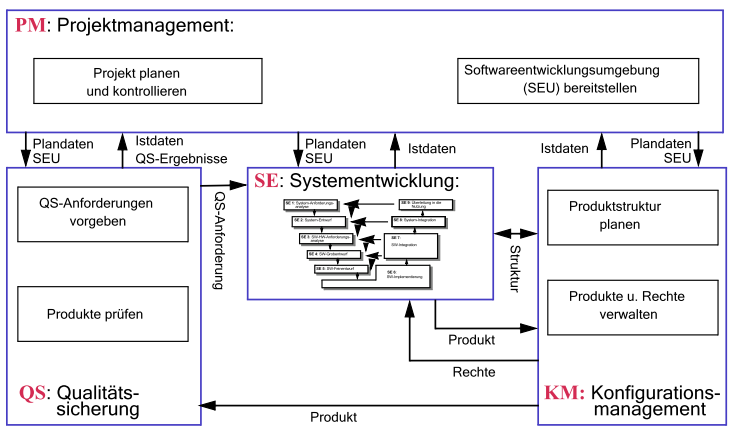
\includegraphics[width=0.85\textwidth]{2_1_1}
\end{figure}
\begin{figure}[h]
	\caption{Grafische Übersicht über Aufgaben- und Rollenverteilung}
	\centering
	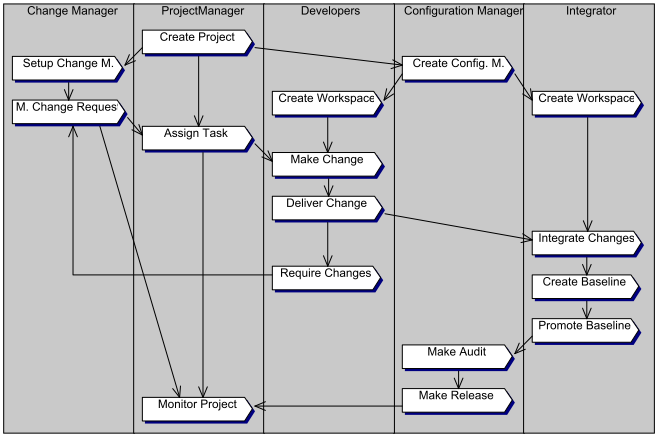
\includegraphics[width=0.85\textwidth]{2_1_2}
\end{figure}
\paragraph{Workspaces für das Konfigurationsmanagement}
\begin{figure}[h]
	\caption{Workspaces für das Konfigurationsmanagement}
	\centering
	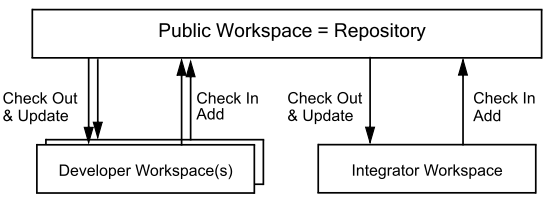
\includegraphics[width=0.6\textwidth]{2_1_3}
\end{figure}
\begin{itemize}
	\item alle Dokumente (Objekte, Komponenten) zu einem bestimmten Projekt werden in	einem gemeinsamen Repository (\textbf{public workspace}) aufgehoben
	\item im Repository werden nicht nur aktuelle Versionen, sondern auch alle \textbf{früheren Versionen} aller Dokumenten gehalten
	\item beteiligte Entwickler bearbeiten ihre eigenen Versionen dieser Dokumente in 
	ihrem privaten Arbeitsbereich (private workspace, \textbf{developer workspace}) 
	\item es gibt genau einen Integrationsarbeitsbereich (\textbf{integrations workspace}) für die Systemintegration
\end{itemize}
\paragraph{Aktivitäten bei der Arbeit mit Workspaces}
\begin{itemize}
	\item Personen holen sich Versionen neuer Dokumente, die von anderen Personen erstellt wurden(\textbf{checkout}), ih ihren privaten Arbeitsbereich
	\item Personen passen ihre Privatversionen ggf. von Zeit zu Zeit an neue Versionen im öffentlichen Repository an (\textbf{update}).
	\item Sie fügen (hoffentlich) nur konsistente Dokumente als neue Versionen in das allgemeine Repository ein (\textbf{checkin = commit}).
	\item Ab und an werden neue Dokumente dem Repository hinzugefügt (\textbf{add}). 
	\item Jede Person kann alte/neue Versionen frei wählen.
\end{itemize}
\paragraph{Probleme}
\begin{itemize}
	\item Wie wird Konsistenz von Gruppen abhängiger Dokumente sichergestellt?
	\item Was passiert bei gleichzeitigen Änderungswünschen für ein Dokument?
	\item Wie realisiert man die Repository-Operationen effizient?
	\item Wie unterstützt man ''Offline''-Arbeit (ohne Zugriff auf Repository)?
\end{itemize}
\paragraph{Weitere Begriffe des Konfigurationsmanagements}
\begin{itemize}
	\item \textbf{Dokument} = Gegenstand, der der Konfigurationsverwaltung unterworfen wird (eine einzelne Datei oder ein ganzer Dateibaum oder ... )
	\item \textbf{(Versions-)Objekt} = Zustand einer Dokument zu einem bestimmten Zeitpunkt in einer bestimmten Ausprägung
	\item \textbf{Varianten} = parallel zueinander (gleichzeitig) existierende Ausprägungen eines Dokuments, die unterschiedliche Anforderungen erfüllen
	\item \textbf{Revisionen} = zeitlich aufeinander folgende Zustände eines Dokuments
	\item  \textbf{Konfiguration} = komplexes Versionsobjekt, eine bestimmte Ausprägung eines Programmsystems (oft hierarchisch strukturierte Menge von Dokumenten)
	\item \textbf{Baseline} = eine Konfiguration, die zu einem Meilenstein (Ende einer Entwicklungsphase) gehört und evaluiert (getestet) wird
	\item \textbf{Release} = eine stabile Baseline, die ausgeliefert wird (intern an Entwickler oder extern an bestimmte Kunden oder ... )
\end{itemize}
\subsection{Versionsmanagement}
Bekannteste ''open source''-Produkte (in zeitlicher Reihenfolge) sind:
\begin{itemize}
	\item Source Code Control System \textbf{SCCS} von AT\&T (Bell Labs):
	\begin{itemize}
		\item effiziente Speicherung von Textdateiversionen als ''Patches''
	\end{itemize}
	\item Revision Control System \textbf{RCS} von Berkley/Purdue University
	\begin{itemize}
		\item schnellerer Zugriff auf Textdateiversionen
	\end{itemize}
	\item Concurrent Version (Control) System \textbf{CVS} (zunächst Skripte für RCS)
	\begin{itemize}
		\item Verwaltung von Dateibäumen
		\item parallele Bearbeitung von Textdateiversionen
	\end{itemize}
	\item Subversion \textbf{SVN} - CVS-Nachfolger von CollabNet initiiert (http://www.collab.net)
	\begin{itemize}
		\item Versionierung von Dateibäumen
	\end{itemize}
	\item \textbf{Git}, Mercurial, ... als verteilte Versionsmanagementsysteme
	\begin{itemize}
		\item jeder Entwickler hat eigene/lokale Versionsverwaltung
	\end{itemize}
\end{itemize}
\subsubsection{Source Code Control System SCCS von AT\&T (Bell Labs)}
Je Dokument (Quelltextdatei) gibt es eine eigene \textbf{History-Datei}, die alle Revisionen als eine Liste jeweils geänderter (Text-)Blöcke speichert:
\begin{itemize}
	\item jeder Block ist ein \textbf{Delta}, das Änderungen zwischen Vorgängerrevision und aktueller Revision beschreibt
	\item jedes Delta hat \textbf{SCCS-Identifikationsnummer} der zugehörigen Revision: <ReleaseNo>.<LevelNo>.<BranchNo>.<SequenceNo>
\end{itemize}
\paragraph{Revisionsbäume von SCSS}
\begin{itemize}
	\item Release 1.1 \ Neuentwicklung
	\item Release 1.1 \ Wartung
	\item Release 1.2 \ Weiterentwicklung
	\item Release 2 \ Weiterentwicklung
\end{itemize}
\paragraph{Erläuterungen zu ''diff'' und ''patch''}
\begin{itemize}
	\item ''\textbf{diff}''-Werkzeug bestimmt Unterschiede zwischen (Text-)Dateien = \textbf{Deltas}
	\item ein Delta(diff) zwischen zwei Textdateien besteht aus einer Folge von ''Hunks'', die jeweils Änderungen eines Zeilenbereichs beschreiben:
	\begin{itemize}
		\item Änderungen von Zeilen: werden mit ''\textbf{!}'' markiert
		\item Hinzufügen von Zeilen: werden mit ''\textbf{+}'' markiert
		\item Löschen von Zeilen: werden mit ''\textbf{-}'' markiert
	\end{itemize}
	\item reale Deltas enthalten unveränderte \textbf{Kontextzeilen} zur besseren Identifikation von Änderungsstellen
	\item ein \textbf{Vorwärtsdelta} zwischen zwei Dateien d1 und d2 kann als ''\textbf{patch}'' zur Erzeugung von Datei d2 auf Datei d1 angewendet werden
	\item inverses \textbf{Rückwärtsdelta} zwischen zwei Dateien d1 und d2 kann als ''patch'' zur Wiederherstellung von Datei d1 auf Datei d2 angewendet werden
	\item SCCS-Deltas sind in einer Datei gespeichert, deshalb weder Vorwärts- noch Rückwärts- sondern \textbf{Inline-Deltas}
\end{itemize}
\paragraph{Genauere Instruktionen zur Erzeugung von Deltas}
Jedes ''diff''-Werkzeug hat seine eigenen Heuristiken, wie es möglichst kleine und/oder lesbare Deltas/Patches erzeugt, die die Unterschiede zweier Dateien darstellen. Ein möglicher (und in den Übungen verwendeter) Satz von Regeln zur Erzeugung von Deltas sieht wie folgt aus:
\begin{enumerate}
	\item Die Anzahl der geänderten, gelöschten und neu erzeugten Zeilen aller Hunks eines \textbf{Deltas} zweier Dateien wird möglichst klein gehalten.
	\item Jeder Hunk beginnt mit genau einer unveränderten \textbf{Kontextzeile} und enthält sonst nur geänderte, gelöschte oder neu eingefügte Zeilen (Ausnahme: Dateianfang).
	\item Aufeinander folgende Hunks sind also durch jeweils \textbf{mindestens eine unveränderte Zeile} getrennt.
	\item Optional: Anstelle von Löschen und Neuerzeugen einer Zeile i verwendet man die 
	\textbf{Änderungsmarkierung ''!''}
\end{enumerate}
\paragraph{Durch diese Regeln nicht gelöstes Problem}
Wie erkenne ich, ob eine Änderung in Zeile i durch Einfügen einer neuen Zeile oder durch Ändern einer alten Zeile zustande gekommen ist?
\paragraph{Create- und Apply-Patch in Eclipse}
Die ''Create Patch''- und ''Apply Patch''-Funktionen in Eclipse benutzen genau das gerade eingeführte ''Unified Diff''-Format. Dabei werden bei der Erzeugung von Hunks wohl folgende Heuristiken/Regeln verwendet:
\begin{itemize}
	\item ein Hunk scheint in der Regel mit drei unveränderten Kontextzeilen zu beginnen (inklusive Leerzeilen).
	\item zwei Blöcke geänderter Zeilen müssen durch mindestens sieben unveränderte Zeilen getrennt sein, damit dafür getrennte Hunks erzeugt werden
\end{itemize}
Bei der Anwendung von Patches werden folgende Heuristiken/Regeln verwendet:
\begin{itemize}
	\item werden der Kontext oder die zu löschenden Zeilen eines Patches so nicht gefunden, dann endet die Patch-Anwendung mit einer Fehlermeldung
	\item befindet sich die zu patchende Stelle eines Textes nicht mehr an der angegebenen Stelle (Zeile), so wird trotzdem der Patch angewendet
	\item gibt es mehrere (identische) Stellen in einem Text, auf die ein Patch angewendet werden kann, so wird die Stelle verändert, die am nächsten zur alten Position ist
\end{itemize}
\paragraph{Eigenschaften von SCSS}
\begin{itemize}
	\item für beliebinge (Text-)Dateien verwendbar (und nur für solche
	\item Schreibsperren auf ''ausgecheckten'' Revisionen
	\item Revisionsbäume mit manuellem Konsistenthalten von Entwicklungszweigen
	\item Rekonstruktionszeit von Revisionen steigt linear mit der Anzahl der Revisionen (Durchlauf durch Blockliste)
	\item Revisionsidentifikation nur durch Nummer und Datum
\end{itemize}
\paragraph{Offene Probleme}
\begin{itemize}
	\item Kein Konfigurationsbegriff und kein Variantenbegriff
	\item Keine Unterstützung zur Verwaltung von Konsistenzbeziehungen zwischen verschiedenen Objekten
\end{itemize}
\paragraph{Probleme mit Schreibsperren}
SCCS realisiert ein sogenanntes ''pessimistisches'' Sperrkonzept. Gleichzeitige Bearbeitung einer Datei durch mehrere Personen wird verhindert:
\begin{itemize}
	\item ein Checkout zum Schreiben (\textbf{single write access})
	\item mehrere Checkouts zum Lesen (\textbf{multiple read access})
\end{itemize}
In der Praxis kommt es aber öfter vor, dass mehrere Entwickler dieselbe Datei zeitgleich verändern müssen (oder Person mit Schreibrecht ''commit'' vergisst...)
\paragraph{Unbefriedigende Lösungen}
\begin{itemize}
	\item Entwickler mit Schreibrecht macht ''commit'' unfertiger Datei, Entwickler mit dringendstem Änderungswunsch macht ''checkout'' mit Schreibrecht
	\begin{itemize}
		\item inkonsistente Zustände in Repository, nur einer darf ''Arbeiten''
	\end{itemize}
	\item weitere Entwickler mir Schreibwunsch ''stehlen'' Datei, machen also ''checkout'' mit Leserecht und modifizieren Datei trotzdem
	\begin{itemize}
		\item Problem: Verschmelzen der verschiedenen Änderungen
	\end{itemize}
\end{itemize}
\subsubsection{Revision Control System RCS von Berkley/Purdue University}Je Dokument (immer Textdatei) gibt es eine eigene History-Datei, die eine neueste Revision vollständig und andere Revisionen als \textbf{Deltas} speichert:
\begin{itemize}
	\item optionale \textbf{Schreibsperren} (verhindern ggf. paralleles Ändern)
	\item \textbf{Revisionsbäume} mit besserem Zugriff auf Revisionen:
	\begin{itemize}
		\item schneller Zugriff auf neueste Revision auf Hauptzweig
		\item langsamer Zugriff auf ältere Revisionen auf Hauptzweig  (mit \textbf{Rückwärtsdeltas})
		\item langsamer Zugriff auf Revisionen auf Nebenzweigen (mit \textbf{Vorwärtsdeltas}).
	\end{itemize}
	\item Versionsidentifikation auch durch frei wählbare Bezeichner
\end{itemize}
\paragraph{Offene Probleme}
Kein Konfigurationsbegriff und kein Variantenbegriff
\begin{figure}[h]
	\caption{Deltaspeicherung von Revisionen als gerichtete Graphen}
	\centering
	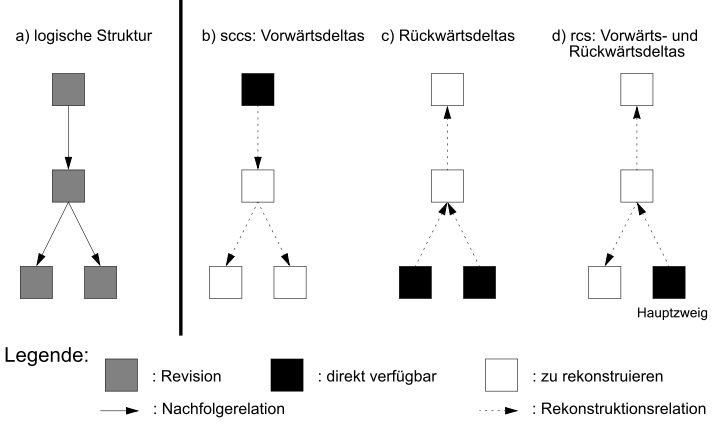
\includegraphics[width=0.85\textwidth]{2_2_1}
\end{figure}
\subsubsection{Concurrent Version (Management) System CVS}
\subsection{Releasemanagement}
\subsection{Buildmanagement}
\subsection{Änderungsmanagement}
\subsection{Zusammenfassung}



